\documentclass[twoside,a4paper]{article}
\usepackage{geometry}
\usepackage{ctex, hyperref}
\geometry{margin=1.5cm, vmargin={0pt,1cm}}
\setlength{\topmargin}{-1cm}
\setlength{\paperheight}{29.7cm}
\setlength{\textheight}{25.3cm}

% useful packages.
\usepackage{amsfonts}
\usepackage{amsmath}
\usepackage{amssymb}
\usepackage{amsthm}
\usepackage{enumerate}
\usepackage{graphicx}
\usepackage{multicol}
\usepackage{fancyhdr}
\usepackage{layout}
\usepackage{listings}%插入代码
\usepackage{ctex}%引入中文包
\usepackage{graphicx}%插入图片的包
\usepackage{geometry}%设置A4纸页边距的包
\usepackage{url}
\usepackage{stfloats}
\usepackage{float}
\usepackage{amssymb}
\usepackage{listings}
% some common command
\newcommand{\dif}{\mathrm{d}}
\newcommand{\avg}[1]{\left\langle #1 \right\rangle}
\newcommand{\difFrac}[2]{\frac{\dif #1}{\dif #2}}
\newcommand{\pdfFrac}[2]{\frac{\partial #1}{\partial #2}}
\newcommand{\OFL}{\mathrm{OFL}}
\newcommand{\UFL}{\mathrm{UFL}}
\newcommand{\fl}{\mathrm{fl}}
\newcommand{\op}{\odot}
\newcommand{\Eabs}{E_{\mathrm{abs}}}
\newcommand{\Erel}{E_{\mathrm{rel}}}

\begin{document}

\pagestyle{fancy}
\fancyhead{}
\lhead{褚朱钇恒 (3200104144)}
\chead{Numerical PDE homework \#3}
\rhead{2023.5.5}

\section{Exercise 11.9}

验证real positivity,由$||T||\ge \inf\{M\ge 0\}=0\Rightarrow ||T||\ge 0$

验证point separation,$||T||=0\Rightarrow \forall x,||Tx||\le M||x||=0\Rightarrow T=0$

验证absolute homogeneity,$\forall a\in \mathbb{F},v\in \mathcal{V}(\mathbb{F}^n,\mathbb{F}^m)$

有$||av||=\inf\{M\ge 0:\forall x\in \mathbb{F}^n,|avx|=|a||vx|\le M|x|\}$

若$|a|=0,||av||=0=|a|||v||$,否则,有$||av||=\inf{M\ge 0:\forall x\in \mathbb{F}^n,|vx|\le \frac{M}{|a|}|x|}$,也有$||av||=|a|||v||$

\

验证triangle inequality,$\forall u,v\in \mathcal{V}(\mathbb{F}^n,\mathbb{F}^m)$


$||u+v||=\inf\{M\ge 0:\forall x\in \mathbb{F}^n,|(u+v)x|=|ux+vx|\le M|x|\}$

设$||u||=M_1,||v||=M_2$,则有$\forall x\in \mathbb{F}^n,|ux|\le M_1|x|,|vx|\le M_2|x|\Rightarrow |ux|+|vx|\le (M_1+M_2)|x|$

有$||u+v||\le M_1+M_2=||u||+||v||$

所以有$||\cdot||$是一个范数

\section{Exercise 11.13}
验证non-negativity,由范数的非负性,$d(S,T)=||S-T||\ge 0$

验证identity of indiscernibles,$d(S,T)=0\Leftrightarrow ||S-T||=0 \Leftrightarrow $

$\forall x |(S-T)x|=0=|Sx-Tx|\Leftrightarrow \forall x Sx=Tx \Leftrightarrow S=T$

\

验证symmetry,$d(S,T)=||S-T||=||T-S||=d(T,S)$

验证triangle inequality,$d(A,B)=||A-B||\le ||A-C||+||C-B||=d(A,C)+d(C,B)$

\section{Exercise 11.16}
real positivity,point separation,absolute homogeneity显然,下证triangle inequality:

\begin{align}
  ||u+v||^2&= \sum_{j=1}^n||ue_j+ve_j||^2\\
  &= \sum_{j=1}^n(||ue_j||^2+||ve_j||^2+2\langle ue_j,ve_j\rangle)\\
  &=||u||^2+||v||^2+2\sum_{j=1}^n\langle ue_j,ve_j\rangle(\mbox{由内积的性质})\\
  &\le ||u||^2+||v||^2+2\sqrt{\sum_{j=1}^n||ue_j||^2||ve_j||^2}(\mbox{由柯西不等式})\\
  &\le ||u||^2+||v||^2+2\sqrt{\sum_{j=1}^n||ue_j||^2\sum_{j=1}^n||ve_j||^2}\\
  &\le ||u||^2+||v||^2+2\sqrt{||u||^2||v||^2}\\
  &\le ||u||^2+||v||^2+2||u||||v||\\
  &\le (||u||+||v||)^2\\
\end{align}

两边同时开平方即可得$||u+v||\le ||u||+||v||$


\section{Exercise 11.20}

由11.18有$|TSx|\le|T||Sx|$

则$|TS|^2=\sum_{j=1}^k||TSe_j||^2\le\sum_{j=1}^k(|T||Se_j||)^2=|T|^2\sum_{j=1}^k(|Se_j||)^2=|T|^2|S|^2$

两边同时开平方即可得$|TS|\le|T||S|$

\section{Exercise 11.36}

设$X=PJP^{-1}$,$J$为约当标准型,$P$为可逆矩阵,则有$det(X)=det(PJP^{-1})=det(P)det(J)det(P^{-1})=det(J)$
且$trace(X)=trace(PJP^{-1})=trace(P)trace(J)trace(P^{-1})=trace(J)$

设X的特征值为$\lambda_1,\dots,\lambda_n$,则有$trace(X)=\Sigma_{i=1}^N\lambda_i$

所以有$det(e^{X})=e^{J}=e^{\Sigma_{i=1}^N\lambda_i}=e^{trace(X)}$

\section{Exercise 11.50}
由于 $v$ 和 $w$ 都满足相同的初值问题,因此我们有:

$$\begin{aligned}
|v(t) - w(t)| &= |v(a) - w(a) + \int_a^t f(v(s),s) - f(w(s),s)ds| \\
&\leq |v(a) - w(a)| + \left|\int_a^t f(v(s),s) - f(w(s),s)ds\right| \\
&\leq |v(a) - w(a)| + L\int_a^t |v(s) - w(s)|ds,
\end{aligned}$$
其中 $L$ 是 $f$ 关于其第一个变量的 Lipschitz 常数。 

于是有
$$
|v(t) - w(t)| -L\int_a^t |v(s) - w(s)|ds \leq |v(a) - w(a)|
$$
$$
(e^{-tL}\int_a^t |v(s) - w(s)|ds)^{'} \leq e^{-tL}|v(a) - w(a)|
$$
两边求积分得
$$
(e^{-tL}\int_a^t |v(s) - w(s)|ds) \leq e^{-tL}|v(a) - w(a)|\frac{e^{-aL}-e^{-tL}}{L}
$$
两边除以$e^{-tL}$再求导即可得到
$$|v(t) - w(t)| \leq |v(a) - w(a)|\exp(L(t-a))$$ 证毕


\section{Exercise 11.100}

对于 trapezoidal rule,$s=1,\alpha_1=1,\alpha_0=-1,\beta_0=\beta_1=\frac{1}{2}$
$$\begin{aligned}
  C_0&=\sum_{j=0}^s\alpha_j=0\\
  C_1&=\sum_{j=0}^s(j\alpha_j-\beta_j)=0\\
  C_2&=\sum_{j=0}^s(\frac{1}{2!}j^2\alpha_j-j\beta_j)=0\\
  C_3&=\sum_{j=0}^s(\frac{1}{3!}j^3\alpha_j-\frac{1}{2!}j^2\beta_j)=-\frac{1}{12}\\
  C_4&=\sum_{j=0}^s(\frac{1}{4!}j^4\alpha_j-\frac{1}{3!}j^3\beta_j)=-\frac{1}{24}\\
  \end{aligned}$$
  对于 midpoint method,$s=2,\alpha_2=1,\alpha_1=0,\alpha_0=-1,\beta_0=0,\beta_1=2$
  $$\begin{aligned}
    C_0&=\sum_{j=0}^s\alpha_j=0\\
    C_1&=\sum_{j=0}^s(j\alpha_j-\beta_j)=0\\
    C_2&=\sum_{j=0}^s(\frac{1}{2!}j^2\alpha_j-j\beta_j)=0\\
    C_3&=\sum_{j=0}^s(\frac{1}{3!}j^3\alpha_j-\frac{1}{2!}j^2\beta_j)=\frac{1}{3}\\
    C_4&=\sum_{j=0}^s(\frac{1}{4!}j^4\alpha_j-\frac{1}{3!}j^3\beta_j)=\frac{1}{3}\\
    \end{aligned}$$
    
\section{Exercise 11.102}
    为了达到三阶精度,有$C_0=C_1=C_2=0$,即

    $\sum_{j=0}^s\alpha_j=0,\sum_{j=0}^s(j\alpha_j-\beta_j)=0,\sum_{j=0}^s(\frac{1}{2!}j^2\alpha_j-j\beta_j)=0$

    等价于$\rho(1)=0,\sigma(1)=\rho^{'}(1),\frac{1}{2}\sigma^{'}(1)=\rho^{'}(1)+\rho^{''}(1)$

\section{Exercise 11.103}
使用以下matlab代码分别计算Adams-Bashforth formulas,Adams-Moulton formulas ,Backward differentiation formulas的系数
\begin{lstlisting}
clc; clear;
format rat;
for s=1:5
    a=zeros(s+1,1);
    co=zeros(s,s);
    rhs=zeros(s,1);
    a(s+1)=1;
    a(s)=-1;
    for q=1:s
        for j=0:s-1
            co(q,j+1)=j^(q-1)/factorial(q-1);
            rhs(q)=rhs(q)+j^(q)/factorial(q)*a(j+1);
        end
        rhs(q)=rhs(q)+s^(q)/factorial(q)*a(s+1);
    end
    b=(co\rhs).'
end
   
for s=1:5
    a=zeros(s+1,1);
    co=zeros(s+1,s+1);
    rhs=zeros(s+1,1);
    a(s+1)=1;
    a(s)=-1;
    for q=1:s+1
        for j=0:s
            co(q,j+1)=j^(q-1)/factorial(q-1);
            rhs(q)=rhs(q)+j^(q)/factorial(q)*a(j+1);
        end
    end
    b=(co\rhs).'
end
    
for s=1:5
    co=zeros(s+2,s+2);
    rhs=zeros(s+2,1);
    for q=0:s
        for j=0:s
            co(q+1,j+2)=j^(q)/factorial(q);
        end
        if(q>=1)co(q+1)=-s^(q-1)/factorial(q-1);end
    end
    co(s+2,s+2)=1;
    rhs(s+2)=1;
    ab=(co\rhs).'
end
    
\end{lstlisting}
结果如下:
\begin{lstlisting}
  AdamsBashforth_co =

       1              0              0              0              0       
      -1/2            3/2            0              0              0       
       5/12          -4/3           23/12           0              0       
      -3/8           37/24         -59/24          55/24           0       
     251/720       -637/360        109/30       -1387/360       1901/720   


AdamsMoulton_co =

       1/2            1/2            0              0              0       
      -1/12           2/3            5/12           0              0       
       1/24          -5/24          19/24           3/8            0       
     -19/720         53/360        -11/30         323/360        251/720   


Backwarddifferentiation_co =

1             -1              1              0              0              0       
2/3            1/3           -4/3            1              0              0       
6/11          -2/11           9/11         -18/11           1              0       
12/25           3/25         -16/25          36/25         -48/25           1   
\end{lstlisting}

\section{Exercise 10.108}
$\rho(z)=-\frac{2}{11}+\frac{9}{11}z-\frac{18}{11}z^2+z^3$

$\sigma(z)=\frac{6}{11}z^3$

根据洛必达法则,$\lim_{z\rightarrow 1}\frac{\frac{\rho(z)}{\sigma(z)}-\log z}{(z-1)^4}=\frac{-120z^{-7}+180z^{-6}-72z^{-5}+6z^{-4}}{24}=-\frac{1}{4}=\frac{C_{p+1}}{\sigma(1)}$


\section{Exercise 10.109}

\section{Exercise 10.113}
  证明$zI-M$的行列式为$z^s+\sum_{i=0}^{s-1}a_iz^i$即可

  则有
    $$\begin{aligned}
        &\det(zI-M)\\
          &= \det\begin{pmatrix}
           z & 0 &  & \\
            & z &  & \\
           \vdots & \vdots & \ddots & -1 \\
           a_0 & a_1+a_0z^{-1} & \cdots & z+a_{s-1}
          \end{pmatrix}\\
        &=det\begin{pmatrix}
           z & 0 & 0 & 0 &\cdots& 0\\
            0 & z & 0 &0 &\cdots & 0\\
            0 & 0 & z & -1 &\cdots & 0\\
           \vdots & \vdots &\vdots &\vdots & \ddots & \vdots \\
           a_0 & a_1+a_0z^{-1}& a_2 + a_1z^{-1}+a_0z^{-2} & a_3&\cdots & z+a_{s-1}
          \end{pmatrix}\\
        \end{aligned}$$
      
        根据同理可去掉副对角线上的其他-1项,则有
        $$\begin{aligned}
          &\det(zI-M)\\
        &det\begin{pmatrix}
            z & 0 & 0 & 0 &\cdots& 0\\
            0 & z & 0 &0 &\cdots & 0\\
            0 & 0 & z & 0 &\cdots & 0\\
           \vdots & \vdots &\vdots &\vdots & \ddots & \vdots \\
           a_0 & a_1+a_0z^{-1}& a_2 + a_1z^{-1}+a_0z^{-2} & a_3+a_2z^{-1} + a_1z^{-2}+a_0z^{-3}&\cdots & z+\sum_{i = 0}^{s-1}a_iz^{i-s+1}
        \end{pmatrix}\\
        &=z^s+\sum_{i=0}^{s-1}a_iz^i
      \end{aligned}$$


\section{Exercise 10.119}
    根据11.76,有
    $$\left[\begin{array}{c}
      y_{s-1} \\
      y_{s-2} \\
      y_{s-3} \\
      \vdots \\
      y_{1} \\
      y_{0}
      \end{array}\right]=\left[\begin{array}{cccccc}
          1 & \theta_{1} & \theta_{2} & \cdots & \theta_{s-2} & \theta_{s-1} \\
          0 & 1 & \theta_{1} & \cdots & \theta_{s-3} & \theta_{s-2} \\
          0 & 0 & 1 & \cdots & \theta_{s-4} & \theta_{s-3} \\
          \vdots & \vdots & \vdots & & \vdots & \vdots \\
          0 & 0 & 0 & \cdots & 1 & \theta_{1} \\
          0 & 0 & 0 & \cdots & 0 & 1
          \end{array}\right] \left[\begin{array}{c}
              \tilde{y}_{s-1} \\
              \tilde{y}_{s-2} \\
              \tilde{y}_{s-3} \\
              \vdots \\
              \tilde{y}_{1} \\
              \tilde{y}_{0}
              \end{array}\right].$$
    假设对于$m>0$,原式在$n=0,...,m+s-1$上成立,下证$n=m+s$时也成立

    由题意有, $y_{n+s} = \psi_{n+s} - \sum_{i=0}^{s-1}\alpha_iy_{n+i}$
    $$\begin{aligned}
      y_{m+s} &= \psi_{m+s} - \sum_{i=0}^{s-1}\alpha_iy_{m+i}\\
      &=\psi_{m+s} - \sum_{i=0}^{s-1}\alpha_i(\sum_{j = 0}^{s-1}\theta_{m+i-j}\tilde{y_j}+\sum_{j=s}^{m+i}\theta_{m+i-j}\Phi_j)\\
      &=\psi_{m+s} - \sum_{j=0}^{s-1}\tilde{y_j}\sum_{i=0}^{s-1}\alpha_i\theta_{m+i-j}-\sum_{j=s}^{m+s-1}\psi_j\sum_{i=0}^{s-1}\alpha_i\theta_{m+i-j}\\
      &=\psi_{m+s} + \sum_{j=0}^{s-1}\tilde{y_j}\theta_{m+s-i} + \sum_{j=s}^{m+s-1}\psi_j\theta_{m+s-j}\\
      &=\sum_{1}^{s-1}\tilde{y_j}\theta_{m+s-j}+\sum_{j=s}^{m+s}\psi_j\theta_{m+s-j}
  \end{aligned}
  $$

  故11.118成立


  \section{Exercise 10.124}

  \section{Exercise 10.141}
  
\begin{figure}[H]
    \centering
    \begin{minipage}[t]{0.3\textwidth}
    \centering
    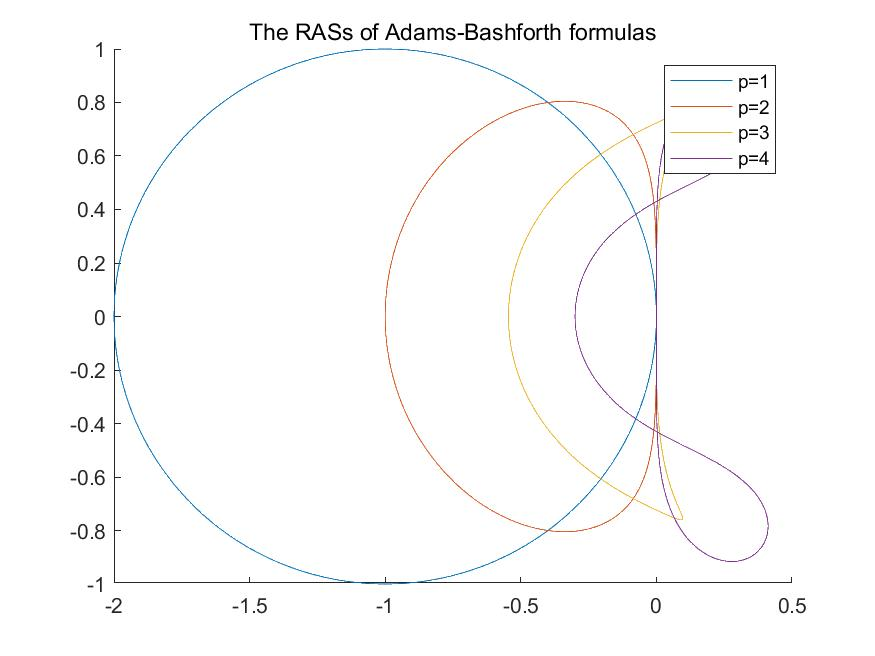
\includegraphics[width=5cm]{./pic/Adams-Bashforth.jpg}
    \end{minipage}
    \begin{minipage}[t]{0.3\textwidth}
    \centering
    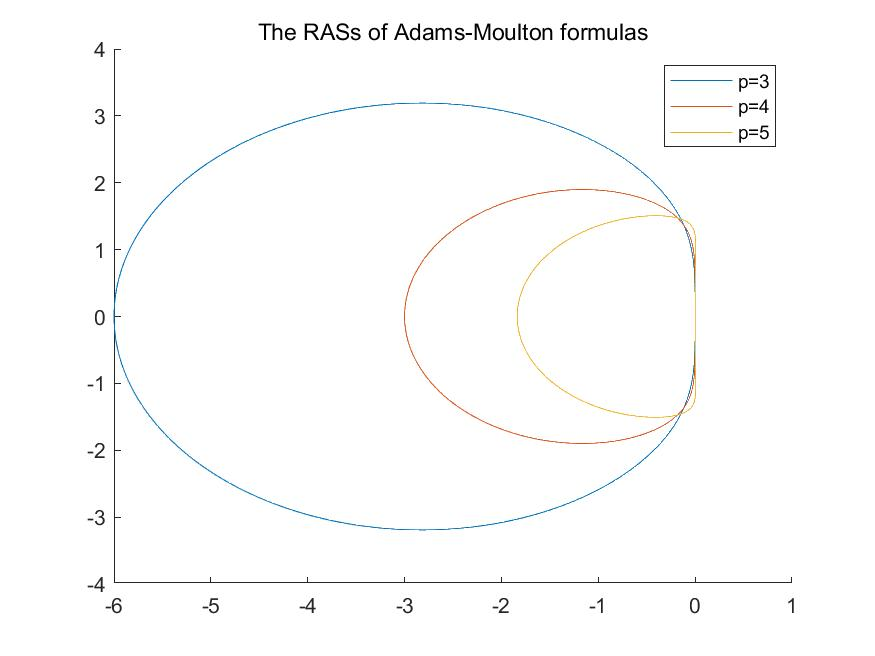
\includegraphics[width=5cm]{./pic/Adams-Moulton.jpg}
    \end{minipage}
    \begin{minipage}[t]{0.3\textwidth}
    \centering
    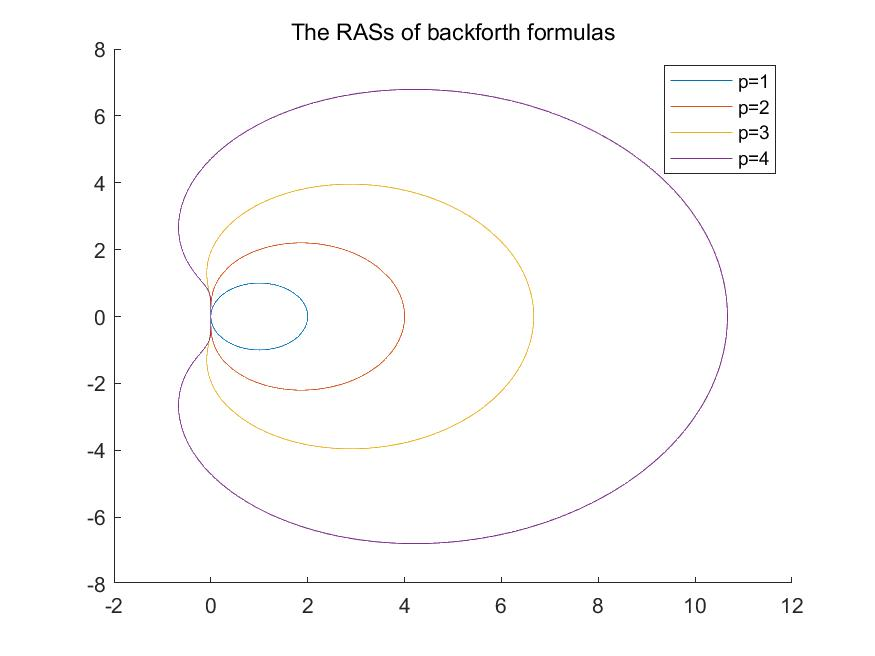
\includegraphics[width=5cm]{./pic/backforth.jpg}
    \end{minipage}
\end{figure}
使用的代码如下:
\begin{lstlisting}
theta = linspace(0, 2*pi, 1000)*1i;
for p=1:4
    hold on;
    z=Adams_Bahsforth_r(p,theta);
    plot(real(z), imag(z));
end
legend('p=1','p=2','p=3','p=4') 
title('The RASs of Adams-Bashforth formulas') 
saveas(gcf, 'Adams-Bashforth.jpg');

cla
for p=3:5
    hold on;
    z=Adams_Moulton_r(p,theta);
    plot(real(z), imag(z));
end
legend('p=3','p=4','p=5') 
title('The RASs of Adams-Moulton formulas') 
saveas(gcf, 'Adams-Moulton.jpg');

cla
for p=1:4
    hold on;
    z=backforth_r(p,theta);
    plot(real(z), imag(z));
end
legend('p=1','p=2','p=3','p=4') 
title('The RASs of backforth formulas') 
saveas(gcf, 'backforth.jpg');
function [re]=Adams_Bahsforth_r(p,theta)
    if(p==1)
        re=exp(theta)-1;
    else if(p==2)
            re=2*(exp(2*theta)-exp(theta))./(3*exp(theta)-1);
        else
            if(p==3)
                re=12*(exp(3*theta)-exp(2*theta))./(23*exp(2*theta)-16*exp(theta)+5);
            else
                if(p==4)
                    re=24*(exp(4*theta)-exp(3*theta))./(55*exp(3*theta)-59*exp(2*theta)+37*exp(theta)-9);
                end
            end
        end
    end
end
function [re]=Adams_Moulton_r(p,theta)
    if(p==3)
        re=12*(exp(2*theta)-exp(theta))./(5*exp(2*theta)+8*exp(theta) - 1);
    else if(p==4)
            re=24*(exp(3*theta)-exp(2*theta))./(9*exp(3*theta)+19*exp(2*theta)-5*exp(theta)+1);
        else
            if(p==5)
                re=720*(exp(4*theta)-exp(3*theta))./(251*exp(4*theta)+646*exp(3*theta)-264*exp(2*theta)+106*exp(theta) - 19);
            end
        end
    end
end

function [re]=backforth_r(p,theta)
    if(p==1)
        re=(exp(theta)-1)./exp(theta);
    else if(p==2)
            re=(3*exp(2*theta)-4*exp(theta)+1)./(2*exp(2*theta));
        else
            if(p==3)
                re=(11*exp(3*theta)-18*exp(2*theta)+9*exp(theta)-2)./(6*exp(3*theta));
            else
                if(p==4)
                    re=(25*exp(4*theta)-48*exp(3*theta)+36*exp(2*theta)-16*exp(theta)+3)./(12*exp(4*theta));
                end
            end
        end
    end
end
\end{lstlisting}

\end{document}